%%% -*-LaTeX-*-

\chapter{Implementation}

In this chapter we will discuss about the implementation details of our system. 

The raw data collected at the routers is exported to Netflow
collectors as described in section 3. NFDUMP \cite{} tools are
used to process the netflow data. They support netflow version v5,v7
and v9. The two tools of primary importance are nfcapd
(netflow capture daemon) that reads the netflow data from
the network and stores the data into files. nfdump (netflow
dump) reads the netflow data from the files stored by nfcapd.
Using nfdump we import the data on to our local machines
from the Netflow Collectors. This imported data forms the
primary source for our experiments. We collect real network
traffic from a campus network with almost XXX users.

Within Feature Engineering we used different python libraries such as NumPy, Spacy and Pandas to clean and manipulate data. Specifically, the mean and median calculating methods from Pandas for missing data and min max scaler, long transformer from NumPys.
For aggregating all the features by a host we used MongoDB to decrease the amount of time it takes for aggregation by indexing \cite{} and inserting the file in database we were able to reduce this steps time from to 20 mts per day. In this context we also wanted to try the approach of streaming algorithms such as bloom filters or count min sketch which gives the aggregate information with little memory foot print which we have xplored a little but left as future work.

As mentioned we have chosen K-Means for our pattern detector and to determine K we used elbow and silhouette approaches. Here we used scikit-learn package implementations of K-Means. To label the behaviors on a given day, we have chosen a reference day and manually labeled its clusters mapping each cluster to a particular behavior as shown in \figref{cluster_comp}.

\begin{figure}[t]
	\centerline{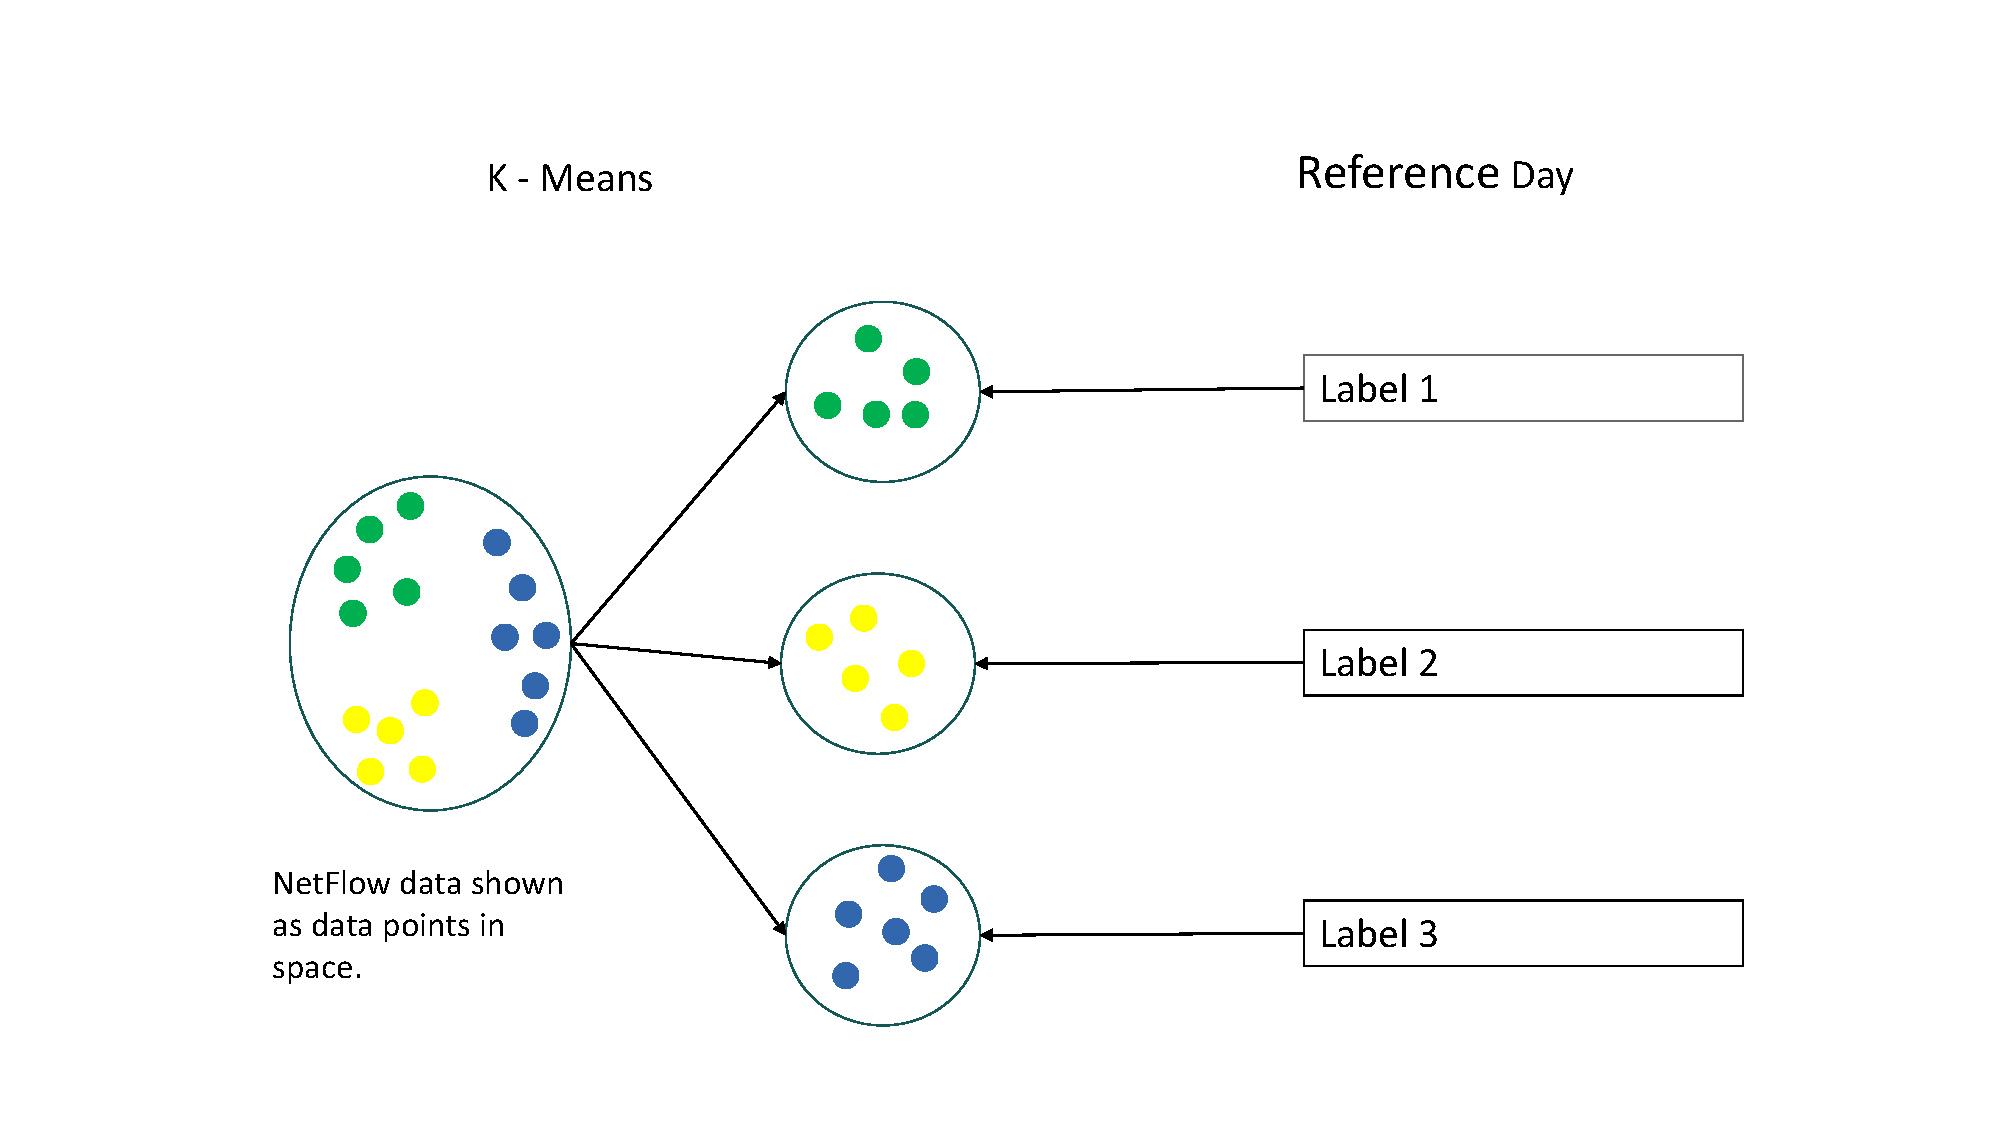
\includegraphics[scale = 0.6]{cluster_comp.pdf}}
	\caption{Process diagram on a reference day, with netflow eight dimensional data aggregated based on host shown as a 2D data point which when passed through our pattern detector split into three clusters. These clusters are manually inspected and labeled accordingly. }%
	\figlabel{cluster_comp}
\end{figure}

 Now for every other day we compare the clusters formed on that given day with the reference day.Cluster comparison is an active research area and there are very few techniques to do this and hence we solved it by converting our cluster comparison problem in to an assignment problem. The assignment problem deals with assigning machines to tasks, workers to jobs, soccer players to positions, and so on. The goal is to determine the optimum assignment that, for example, minimizes the total cost or maximizes the team effectiveness. The assignment problem is a fundamental problem in the area of combinatorial optimization. Assignment problem has polynomial time implementations and one of them is Hungarian Algorithm \cite{}.  In our case the assignment problem is as follows \figref{assign_prob}. On any given day we pass the NetFlow data through patteren detector which will give us clusters on that day, now we map these clusters to the clusters formed on the reference day and subsequently the labels of the reference day clusters gets assigned to the clusters on the given day. 
 
\textit{Hungarian Algorithm}, we use hungarian algorithm to map the clusters formed on two different days. As per this algorithm a cluster on a given day gets mapped to the cluster on a reference day based on the amount of effort it takes to move all the data points from this cluster to the reference day clusters center. Overall this algorithm makes the assignments in such a way that the total effort is least.
  
 
 \begin{figure}[t]
 	\centerline{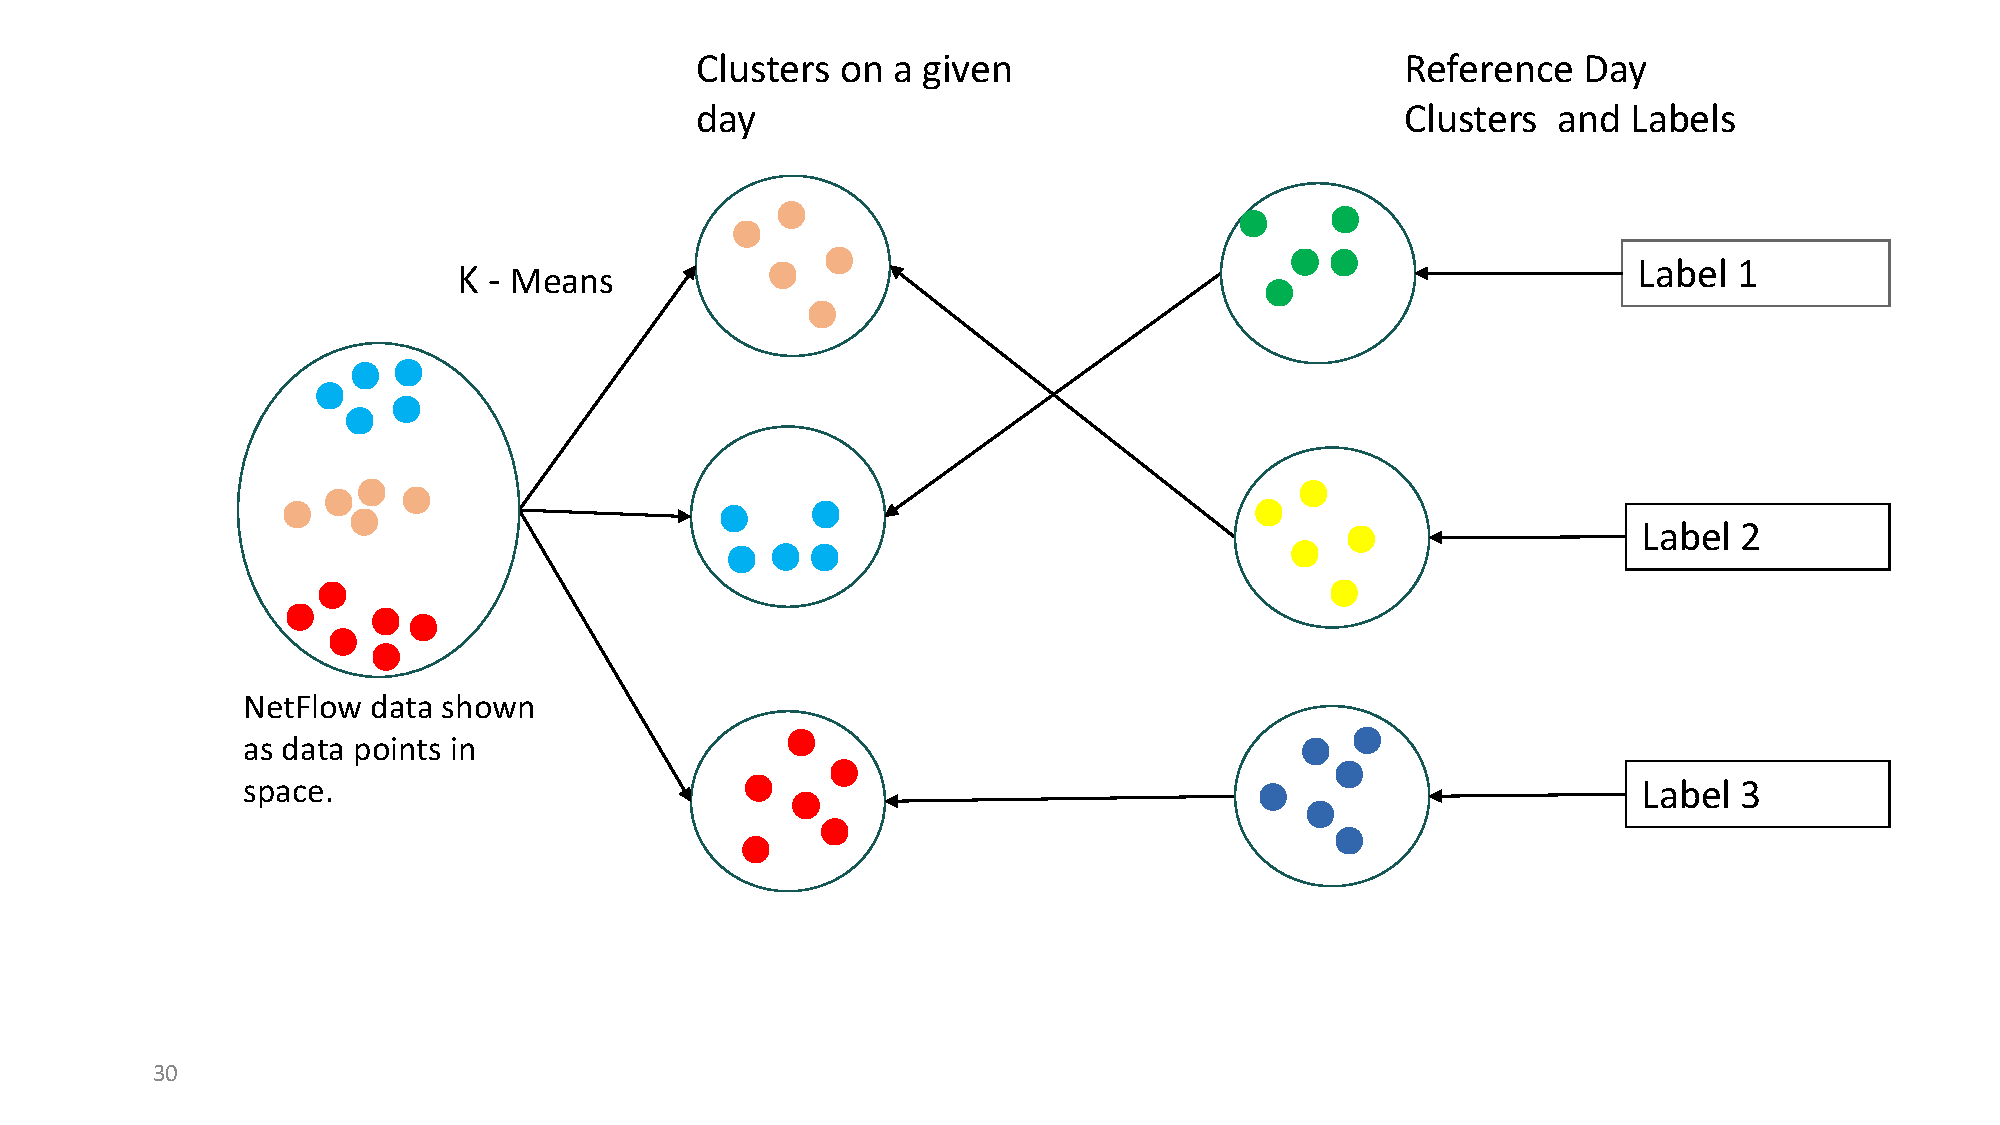
\includegraphics[scale = 0.55]{assign_prob.pdf}}
 	\caption{Process diagram on a reference day, with netflow eight dimensional data aggregated based on host shown as a 2D data point which when passed through our pattern detector split into three clusters. These clusters are manually inspected and labeled accordingly. }%
 	\figlabel{assign_prob}
 \end{figure}

% WE can write about why we ended up with log normalization%
% Also ask rob about what else should go into impl %
% Few numbers like number of code lines, programming languages used, machines on which or code is run machines on which the data is collected, data size every day, execution time for each step after the nfdump we again have manual scripts to move data to other machines and from there we captre it in csv file. here these scripts are also used to feed the data into solarwinds like applications  %
 